\subsection{Colour Swap}\label{sec:colorSwap}
To resolve this issue, the class diagram is used to identify a connection between the preview button and the draw view, which can be seen \figref{figure:class-diagram-colour-swap}.
Two connections are found between \textit{DrawView} and \textit{PreviewButton}, which is \textit{ColorButton} and \textit{DrawFragment}.
\textit{ColorButton} is used when picking a new colour, and assigns the new colour to \textit{PreviewButton}.
However, when pressing the \textit{PreviewButton}, no connection existed.
In order to correct this issue, the event for touching \textit{PreviewButton} could be accessed from \textit{DrawFragment} and was already implemented for the other buttons. 

\begin{figure}[h]
	\centering
	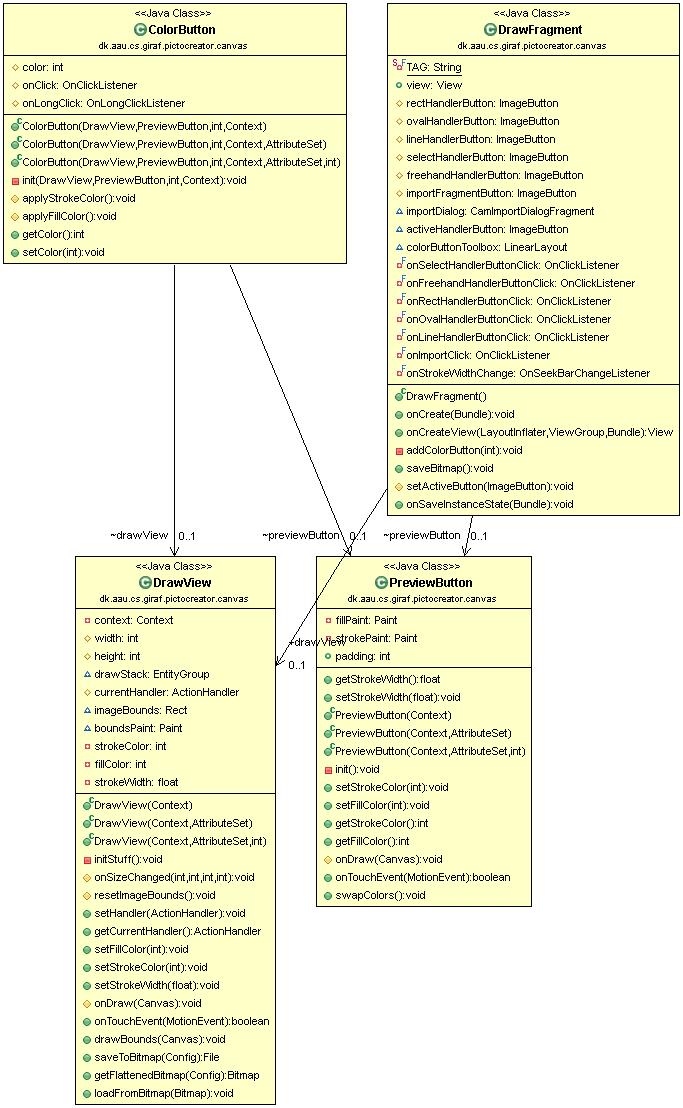
\includegraphics[scale = 0.5]{media/classdiagram-swapcolour-issue}
	\caption{Part of the class diagram.}
	\label{figure:class-diagram-colour-swap}
\end{figure}

In order to correct this issue, the \textit{onTouch} event is moved from \textit{PreviewButton} to \textit{DrawFragment}, since \textit{DrawFragment} has access to both \textit{DrawView} and \textit{PreviewButton}.
\textit{DrawFragment} was already subscribed to the other buttons, thus it is a logical change to move the touch event of \textit{PreviewButton} to \textit{DrawFragment}.
The event implemented in \textit{DrawFragment} can be seen in \lstref{lst:event-previewbuttonclick}.

\begin{lstlisting}[caption={onPreviewButtonClick event},label=lst:event-previewbuttonclick]
private final OnClickListener onPreviewButtonClick = new OnClickListener() {
    @Override
    public void onClick(View v) {
       previewButton.swapColors();
       drawView.setFillColor(previewButton.getFillColor());
       drawView.setStrokeColor(previewButton.getStrokeColor());
    }
};
\end{lstlisting}


\subsubsection{Freehand Drawing Colour}
Before the colour swap functionality was implemented, it was not possible to change the colour of the freehand drawing.
However, with that feature implemented, a bug occurred when using the preview button to swap colours after drawing a freehand drawing. 
By using the button it resulted in swapping the colour of the latest freehand drawing. 
The bug happened since the latest drawn freehand entity was not released after being drawn.
It was not released for the freehand entity, since it overrode that functionality from the superclass, and as of such it had to be added.